\section{Entwicklung von UI-Tests}


Die Entwicklung von UI-Tests ist der zentrale Punkt dieser Arbeit. Im
Gegensatz zu Performance- und Sicherheitstests, die nicht funktional sind,
ist das Hauptziel dieser UI-Tests festzustellen, ob die beiden Versionen von
jExam so funktionieren, wie die Entwickler es beabsichtigt haben.
Dieses Kapitel konzentriert sich auf die Entwicklung der UI-Tests, die
verschiedenen Tools und die Design Patterns, die verwendet wurden. Zunächst
werden die verschiedenen Werkzeuge vorgestellt, die bei der Entwicklung
verwendet wurden. Anschließend werden die Design Patterns vorgestellt, die
dabei helfen, den Code robust und leicht wartbar zu machen. In Teil drei
wird der Schwerpunkt auf die Implementierung von Tests gelegt, und im letzten
Teil werden die erzielten Ergebnisse und zusätzliche Funktionen vorgestellt.

\subsection{Verwendete Werkzeuge}

\subsubsection{Selenium Webdriver}

Selenium ist ein Open-Source-projekt für eine Reihe von Tools und Bibliotheken
zur Unterstützung der Webbrowser-Automatisierung (vgl. \cite{selenium-survey}).
Selenium bietet  Werkzeuge zur Erstellung funktionaler Tests, ohne dass eine
Testskriptsprache erlernt werden muss. Außerdem bietet es eine testspezifische
Sprache (Selenese), mit der Tests in einer Reihe beliebter Programmiersprachen
geschrieben werden können, darunter JavaScript (Node.js), C#, Groovy, Java,
Perl, PHP, Python, Ruby und Scala. Die Tests können dann mit den meisten
modernen Webbrowsern ausgeführt werden. Selenium läuft auf Windows, Linux
und macOS. Selenium besteht aus mehreren Komponenten, von denen jede eine
bestimmte Rolle bei der Entwicklung der Testautomatisierung von Webanwendungen
übernimmt. Zu diesen Komponenten gehören: die Selenium IDE, Selenium Client API,
Selenium Remote Control, Selenium Grid und schließlich der Selenium WebDriver,
der in dieser Arbeit verwendet wird.

Das Kernelement von Selenium ist Selenium WebDriver, eine Schnittstelle zum
Schreiben von Anweisungen, die in verschiedenen Browsern austauschbar sind.
Selenium WebDriver nimmt Befehle entgegen (die in \gls{selenese} oder über eine
Client-API gesendet werden) und sendet sie an einen Browser. Dies wird durch
einen browserspezifischen Browsertreiber implementiert, der Befehle an einen
Browser sendet und Ergebnisse abruft. Die meisten Browsertreiber starten
tatsächlich eine Browseranwendung (z. B. Firefox, Google Chrome, Internet
Explorer, Safari oder Microsoft Edge) und greifen darauf zu. Selenium WebDriver
benötigt keinen speziellen Server, um Tests auszuführen. Stattdessen startet
der WebDriver direkt eine Browserinstanz und steuert sie.  Wo immer möglich,
verwendet WebDriver native Funktionen auf Betriebssystemebene und nicht
browserbasierte JavaScript-Befehle zur Steuerung des Browsers. Dadurch werden
Probleme mit subtilen Unterschieden zwischen nativen und JavaScript-Befehlen,
einschließlich Sicherheitseinschränkungen, vermieden (vgl. \cite{Stewart2016}).
Selenium WebDriver ist vollständig implementiert und wird in JavaScript
(Node.js), Python, Ruby, Java, Kotlin und C# unterstützt.


Selenium ist derzeit das von Testern am meisten geliebte Framework für
UI-Testing (vgl. \cite{selenium-survey} , S. 08-09). Es hat viele Vorteile,
wie z.B. die \"Ubertragbarkeit auf alle Systeme, die einfache Integration mit
andere Technologien, eine große und dynamische Entwicklergemeinschaft sowie
die Dokumentation und die Fülle an verfügbaren Ressourcen. Im Rahmen dieser
Arbeit wird der Selenium Web Driver mit der Programmiersprache Java verwendet.
\subsubsection{TestNG}

TestNG ist ein Open-Source-Testautomatisierungs-Framework für Java. Es wird
nach dem Vorbild von JUnit und NUnit entwickelt. Einige fortgeschrittene und
nützliche Funktionen, die TestNG bietet, machen es zu einem robusteren
Framework im Vergleich zu seinen Mitbewerbern (vgl. \cite{browserstack}).
Das NG in TestNG steht für "Next Generation". Es wird immer häufiger von
Entwicklern und Testern bei der Erstellung von Testfällen verwendet, da es
einfach ist, mehrere Annotationen, Gruppierungen, Abhängigkeiten,
Priorisierungen und Parametrierungsfunktionen zu verwenden. Durch die
Beseitigung der meisten Einschränkungen des älteren Frameworks gibt TestNG
dem Entwickler die Möglichkeit, flexiblere und leistungsfähigere Tests zu
schreiben.

Der Hauptgrund, warum TestNG für die Entwicklung der Tests in dieser
Arbeit ausgewählt wurde, ist in erster Linie die Tatsache, dass es im
Vergleich zu seinem Konkurrenten JUnit mehr nützliche Funktionen
bietet (vgl. \cite{browserstack}):

\begin{enumerate}
    \item Annotationen von TestNG sind im Vergleich zu JUnit
    einfacher zu verstehen
    \item TestNG erfordert im Gegensatz zu JUnit keine
    obligatorische Deklaration von @BeforeClass und @AfterClass
    \item Die Funktion der Parametrisierung, die TestNG bietet, ist
    bequemer und einfacher durch den Datenprovider zu nutzen.
    \item Funktionen wie Priorisierung und Gruppierung von Tests,
    die von TestNG bereitgestellt werden, machen es im Vergleich zu
    JUnit realistischer und leichter anpassbar.
    \item TestNG bietet im Vergleich zu JUnit in mehrfacher
    Hinsicht die Möglichkeit der parallelen Testausführung.

\end{enumerate}

Neben diesen Vorteilen gegenüber JUnit lässt sich TestNG leicht in das
Selenium-Framework integrieren. Dies macht es zu einem der am häufigsten
verwendeten Werkzeuge für das Schreiben von Selenium-Testskripten
(vgl. \cite{selenium-survey}, S.13).

\subsection{Entwurfsmuster}\label{subsec:entwurfsmuster}


Zu den Voraussetzungen, die von der Testinfrastruktur erwartet werden,
gehört die Hohe Wartbarkeit der Testsuite. Dieses Ziel könnte ohne die
Verwendung von Entwurfsmustern nicht erreicht werden. Entwurfsmuster
können den Entwicklungsprozess beschleunigen, indem sie getestete, bewährte
Entwicklungsparadigmen bereitstellen. Ein effektiver Softwareentwurf
erfordert die Berücksichtigung von Problemen, die möglicherweise erst
später bei der Implementierung sichtbar werden. Die Wiederverwendung von
Entwurfsmustern hilft, subtile Probleme zu vermeiden, die zu großen
Problemen führen können, und verbessert die Lesbarkeit des Codes für
Programmierer und Architekten, die mit den Mustern vertraut sind.  Für die
Entwicklung von Tests mit Selenium gibt es zwei Entwurfsmuster, die sehr
beliebt sind und von Testern verwendet werden :
\textbf{Page Object} und \textbf{Factory} (vgl. \cite{pattern-browser}).

\subsubsection{Page Object Model}

Page Object Model ist ein in Selenium verwendetes Entwurfsmuster,
bei dem ein Objektrepository zur Speicherung von WebElementen
erstellt wird. Es wird eine Java-Klasse erstellt, die jeder WebSeite
entspricht (siehe \Cref{fig:page-obj}). Diese Seiten bestehen aus WebElementen und den
entsprechenden Methoden, die auf diese Elemente einwirken (siehe \Cref{fig:page-exp}).
Alle Webseitenelemente befinden sich in einer Java-Klasse, indem sie durch
ihre Locators identifiziert werden.  Darüber hinaus werden für die
verschiedenen Seiten der Webseite mehrere Java-Klassen erstellt. Diese
Java-Klassen dienen als Repository, in dem die verschiedenen Elemente
gespeichert werden, mit denen Testfällen interagieren können. Die Verwendung
des Page Object Model hat viele Vorteile:

\begin{enumerate}
    \item \textbf{Erleichtert die Wartung des Codes} : Da die Testklassen von den
    Klassen getrennt sind, die die Webelemente und die Operationen auf
    ihnen enthalten, ist die Aktualisierung des Codes sehr einfach, wenn
    ein Webelement aktualisiert oder ein neues hinzugefügt wird.
    \item \textbf{Erleichtert die Lesbarkeit des Codes} : Der Benutzer kann das Projekt
    und die Testskripte aufgrund der feinen Trennung zwischen den Testklassen
    und den verschiedenen Webseiten leicht durchlesen.
    \item \textbf{Wiederverwendbarkeit des Codes} : Wenn mehrere Testskripte dieselben
    Webelemente verwenden, müssen nicht in jedem Testskript Code zur
    Behandlung des Webelements geschrieben werden. Die Unterbringung in einer
    separaten Seitenklasse macht es wiederverwendbar, indem es von jedem
    Testskript aus zugänglich gemacht wird.
\end{enumerate}

\begin{figure}[H]
    \centering
    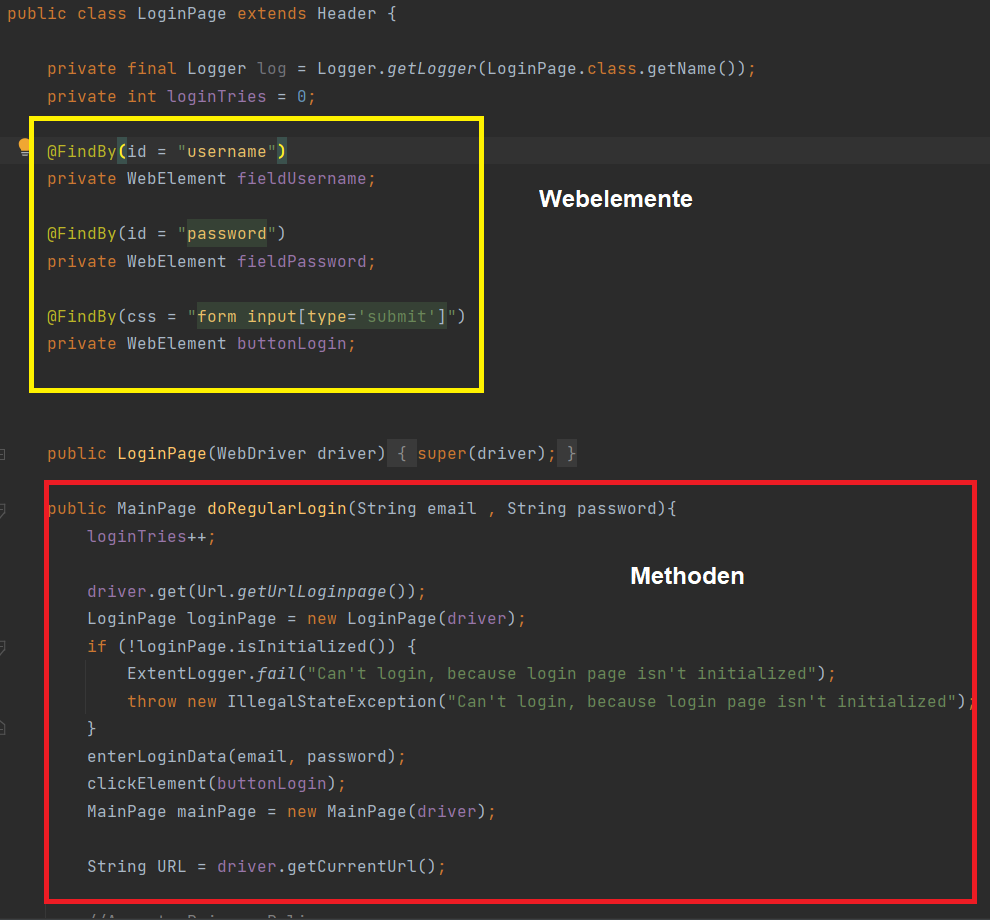
\includegraphics[scale=0.5]{images/page-example}
    \caption{Darstellung der jExam LoginPage mit dem Page Object Model} \label{fig:page-exp}
\end{figure}

\begin{figure}[H]
    \centering
    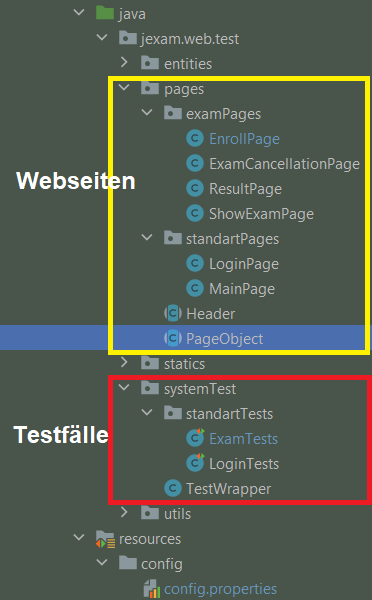
\includegraphics[scale=0.6]{images/page-object}
    \caption{Projektstruktur von jExam Page Object Model} \label{fig:page-obj}
\end{figure}

\subsubsection{Factory}

Page Factory ist eine Klasse, die von Selenium WebDriver bereitgestellt
wird, um das Page Object Model zu implementieren. Das Page Object
Repository wird mit Hilfe des Page Factory-Konzepts von den Testmethoden
getrennt. Page Factory bietet Annotationen, um Elemente zu initialisieren und sie
anschaulich und lesbar macht. Zu den Vorteilen seiner Verwendung gehören:

\begin{enumerate}
    \item \textbf{Sauberer Code}: Das definierte Webelement wird von den Methoden
    getrennt, um eine Webseite in einer Page Object sauber und
    aufgeräumt zu gestalten.
    \item \textbf{Lesbar und beschreibend}: Ein Webelement wird als Variable
    (bekannt als Object Field) deklariert, und die Field-Annotation
    (@FindBy siehe \Cref{fig:page-exp}) wird verwendet, um den Namen, den Typ und
    die Position des Elements zu beschreiben. Auf diese Weise können
    definierte Webelement anhand seiner Annotationen wie Name, Typ
    usw. leicht identifiziert werden.
    \item \textbf{Einfache Wartbarkeit}: Das definierte Webelement kann ohne
    Neudefinition überall in der Page Object Klasse und den Unterklassen
    verwendet werden. Das bedeutet, dass ein bestimmtes Webelement
    mehrmals verwendet werden kann, aber nur an einer Stelle
    definiert ist.
\end{enumerate}


Im nächsten Teil werden die Implementierung der Tests und die verwendeten
Methoden genauer beschrieben.





